% !TEX root=../thesis.tex

\chapter{Background}
\label{chapter:background}

A train network is a complex system. Almost every running train have the 
possibility to affect almost every other train running in the system.  When 
you look at a busy area, such as a major city and it's closest
area, a great deal of trains can be on the move at any given time on a
railway network with limited capacity. This leads to limited time slots for each 
train and every problem can lead to major delays.


Even though one train may be experiencing delay, this delay may be part of a
sequence of problems that can be tracked back to a seemingly unrelated part of
the the network and a perhaps a bad decision there\cite{cule2011mining}. \\

In the Norwegian railroad a train is on schedule if it arrives the final
destination within a margin on 3 minutes and 59 seconds, if it is a long
distance train the margin is 5 minutes and 59 seconds. 
Jernbaneverket (see\vref{subsection:jernbaneverket}) defines regularity as the number of trains that gets run as 
planed in the time schedule. 
Uptime in regards to punctuality is defined by Jernbaneverket from the hours of delay\footnote{Hours of delay due to infrastructure excluded traffic	management and external conditions} caused by infrastructure relative to sum of planed train hours\footnote{Planed train hours (passenger and freight trains)} per year.
\cite{jernbaneverketPunklighetsTall}
\begin{equation} Uptime =
		\frac
				{
					\text{Train hours - Hours of delay}
				}
				{
					\text{Train hours}
				}\times 100 
\end{equation}\\

As Landex\cite{landex2009gis} says, there exist few GIS-approaches concerning
visualization of railroad capacity. Both the visualizations shown by Landex and
in Section \vref{section:backgroundExamples} only seems to take into consideration if
the trains are delayed, and the amount of delay. 

However, to minimize the delays all over the railway network, it may be necessary
to not only see that certain routes are delayed but also why it is delayed. To
be able to understand this, you need to be able to mine data from the railway
network administrator and have a good visualization tool to present it. 

\pagebreak
\section{Examples}
\label{sect:backgroundExamples}

\subsection{Zugmonitor}
\label{sub:subsection_zugmonitor}

In the Zugmonitor (see \vref{fig:zugmonitor}) example each long-distance 
trains in the German railway network has been plotted as a arrow on a German 
map. To illustrate the punctuality of each train, a colored circle has been 
added to each arrow if the train is delayed with varying color depending on 
how big the delay is. It has also been implemented a time line functionality 
to see how the trains are on each step of the routes. This time line 
functionality has both a play forward function and manually drag along the 
time line.

\begin{figure}[!htbp]
	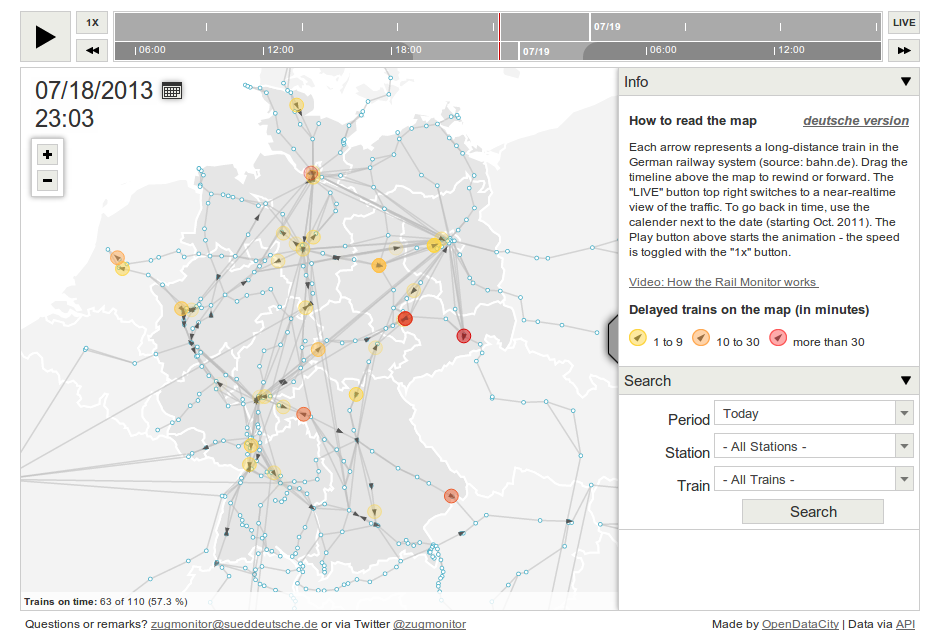
\includegraphics[width=\textwidth,center]{zugmonitor.png}
	\caption[Zugmonitor]{Zugmonitor \cite{zugmonitor}}
	\label{fig:zugmonitor}
\end{figure}
\pagebreak

\subsection{Vaguely live map of trains in the United Kingdom}
\label{sub:subsection_ukLiveMap}

This is a map which plots the relative location of each train in the United
Kingdom (see \vref{fig:ukLiveMap}). The plot fetches the departure time from the 
National Rail website and calculates the relative location. The plot does not
indicate whether or not the trains are on schedule or delayed, this must be
done either manually or for instance checking a time table\cite{trainTimesUK}.
Both the map and time table is developed on hobby basis by the same person. 

\begin{figure}[!htbp]
	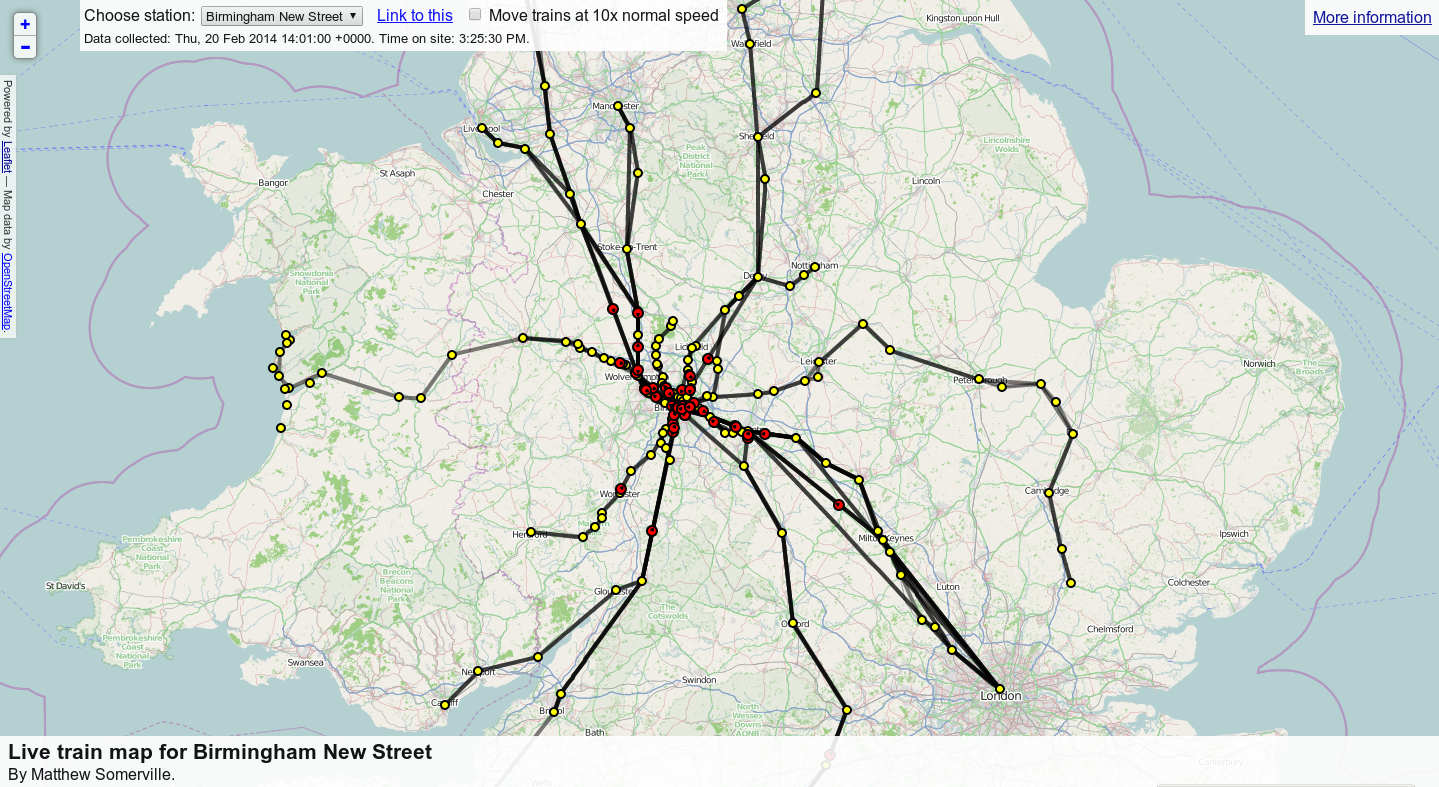
\includegraphics[width=\textwidth,center]{live-train-map-for-Birminingham-new-street.png}
	\caption[Vaguely live map of trains in the United Kingdom]{Vaguely live map of trains in the United Kingdom \cite{ukLiveMap}}
	\label{fig:ukLiveMap}
\end{figure}
\pagebreak

\subsection{MUNI Light Rail}
\label{sub:subsection_muniLightRail}

This a train graph based on the N-Judah line on the Muni Metro light railway line in San Francisco (see \vref{fig:muniLightRail}). 
This chart plots the schedule of the each train and the actual time each train 
uses. The chart auto updates each 10 seconds, and combined with being able 
to spot the difference between the schedule and the actual time, makes it easy 
spot the delay of each train. As with \vref{subsection:ukLiveMap} it has been 
developed on a hobby basis.

\begin{figure}[!htbp]
	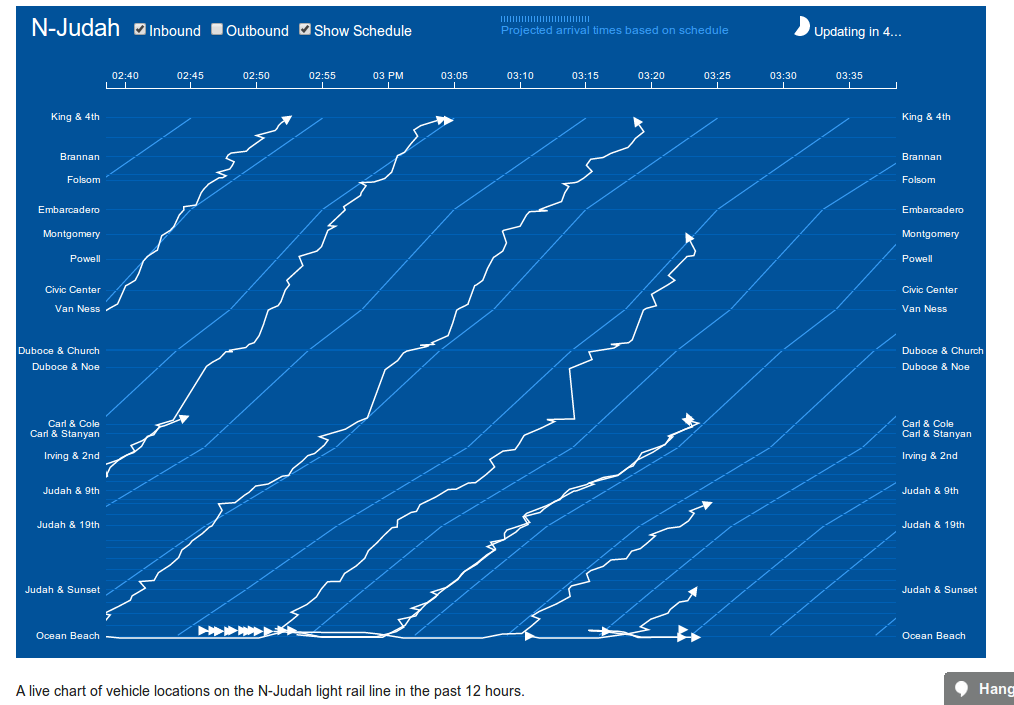
\includegraphics[width=\textwidth,center]{visualizing-transit-delays.png}
	\caption[Visualizing transit delays]{Visualizing transit delays \cite{muniLightRail}}
	\label{fig:muniLightRail}
\end{figure}
\pagebreak


\subsection{MiseryMap}
\label{sub:subsection_zugmonitor}

The MiseryMap (see \vref{fig:miserymap}) shows how much different airports and 
the routes between them are delayed. It also have a playback function to see
how the delays are throughout the day. This plot also shows some weather so it
may be possible to spot if the delays to be blamed on uncontrollable
conditions. 

\begin{figure}[!htbp]
	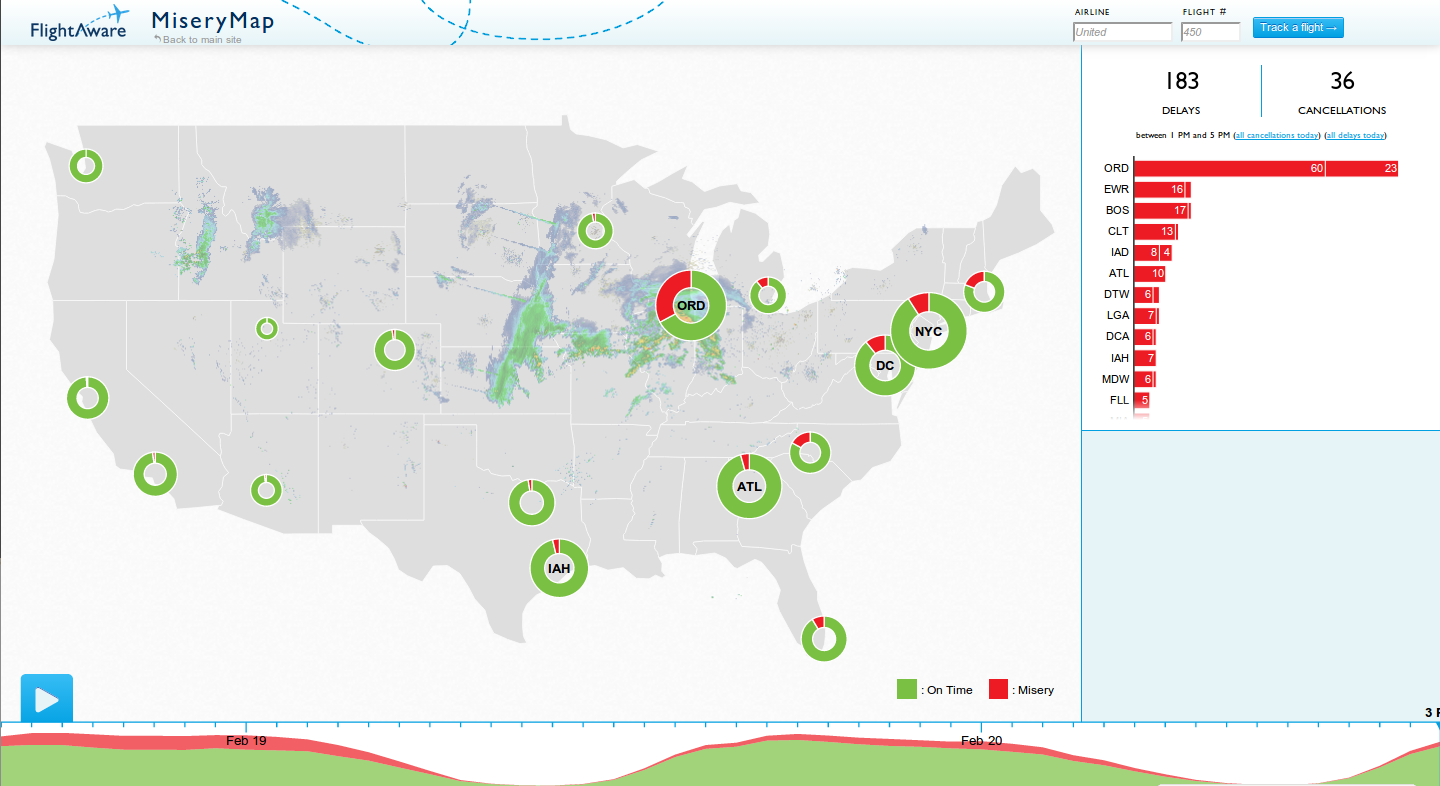
\includegraphics[width=\textwidth,center]{MiseryMap.png}
	\caption[MiseryMap]{MiseryMap \cite{flightAware:MiseryMap}}
	\label{fig:miserymap}
\end{figure}
%\pagebreak
 
\subsection{Jernbaneverket}
\label{sub:subsection_jernbaneverket}

Jernbaneverket is the Norwegian governments agency for railway services \cite{jernbaneverketAbout}.
This means that they are responsible for all the railway network in Norway.
Because of this, they also collect in data from points that each train passes. 
Based on this, they are in the process of releasing a map (see \vref{fig:jernbaneverket-punklighet}) over the punctuality on each stretch. This is a 
interactive map which shows a pop-up box containing the punctuality of the 
stretch clicked on, and this pop-up also shows which routes are using this 
stretch. The map, does not however, show more information if the user zooms 
inn, which is possible within the map itself, and has a static view of Norway 
and the railway.

\begin{figure}[!htbp]
	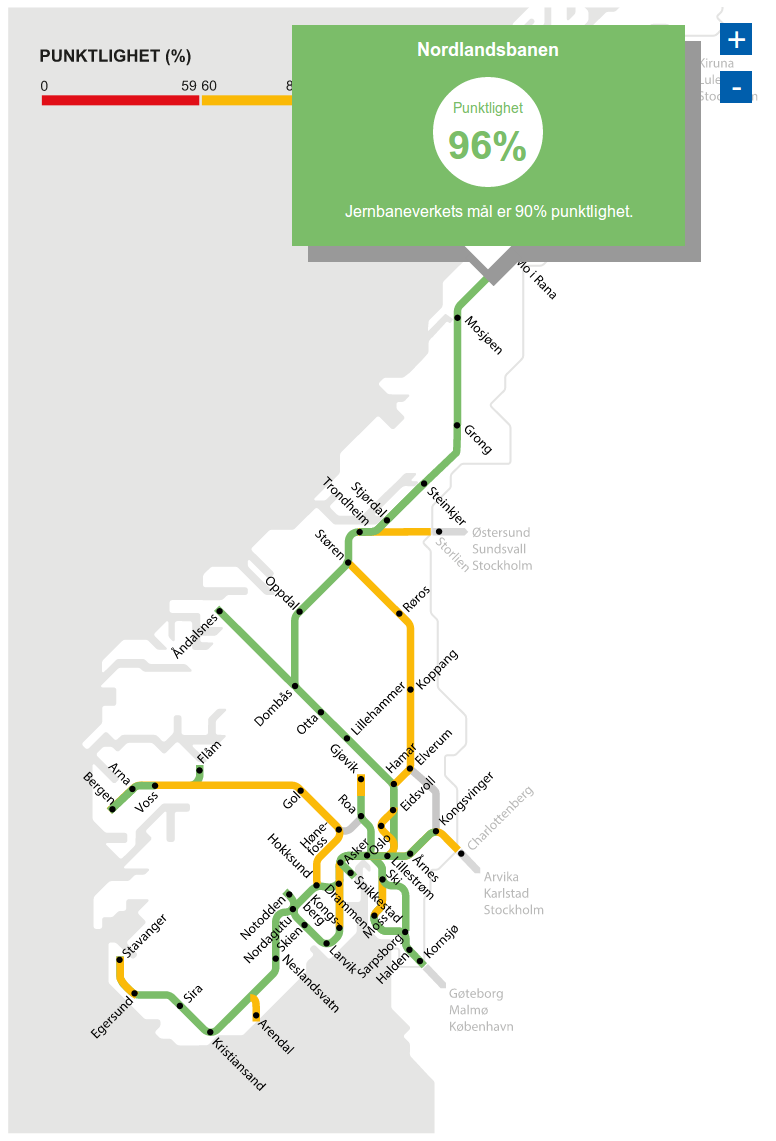
\includegraphics[height=\textheight,center]{jernbaneverket-punklighet.png}
	\caption[Punctuality map for Norwegian railway]{Punctuality map for Norwegian railway
	\cite{jernbaneverketPunklighetKart}}
	\label{fig:jernbaneverket-punklighet}
\end{figure}
\pagebreak


\subsection{Tåg.info}
\label{sub:subsection_taag.info}



\begin{figure}[!htbp]
	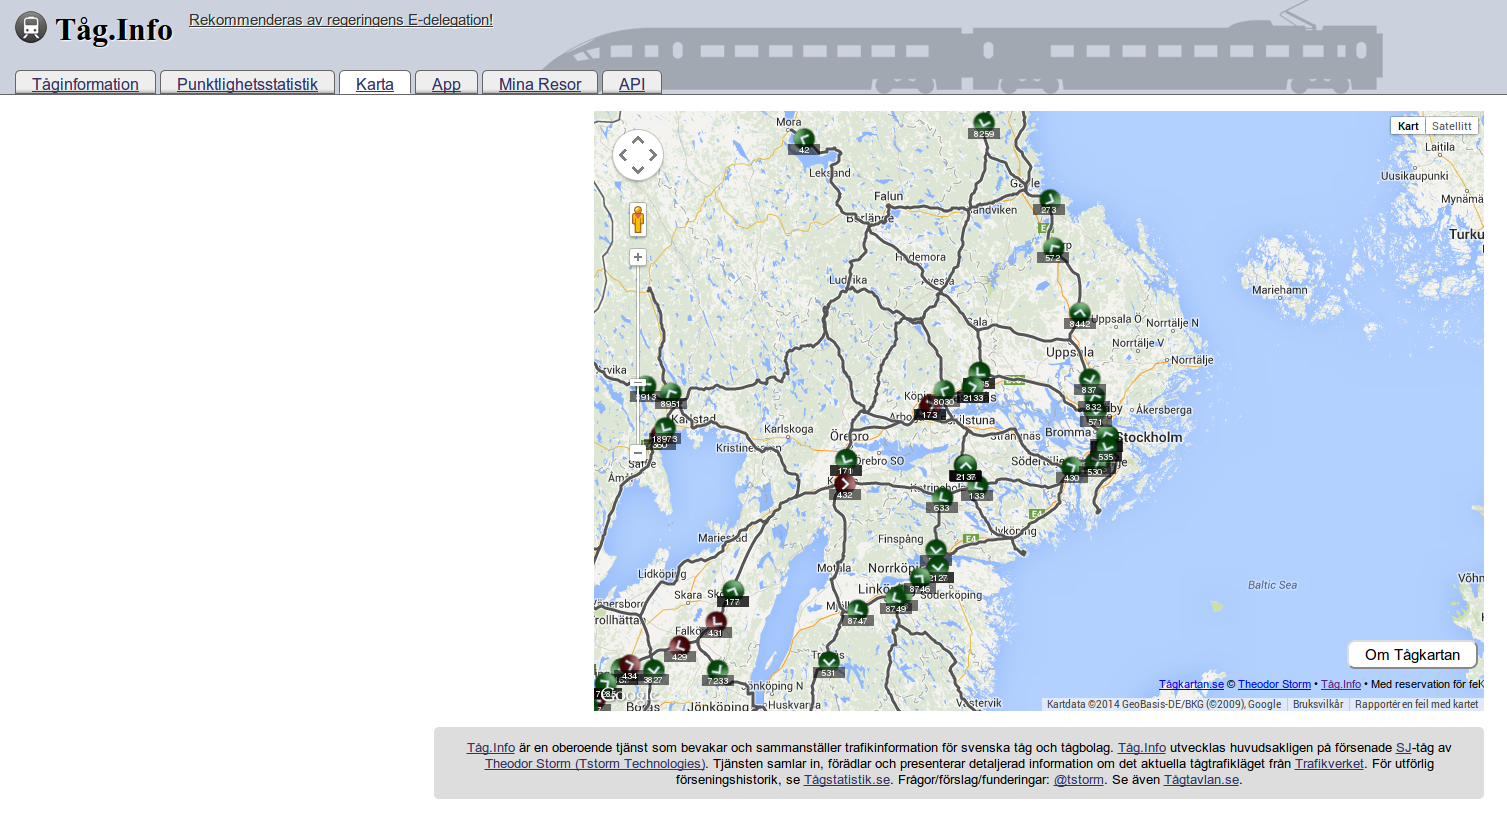
\includegraphics[width=\textwidth,center]{taag-info-kart.png}
	\caption[Tåg.info kart]{Tåg.info kart
	\cite{taagInfo}}
	\label{fig:taag-info-kart}
\end{figure}
\pagebreak

\begin{figure}[!htbp]
	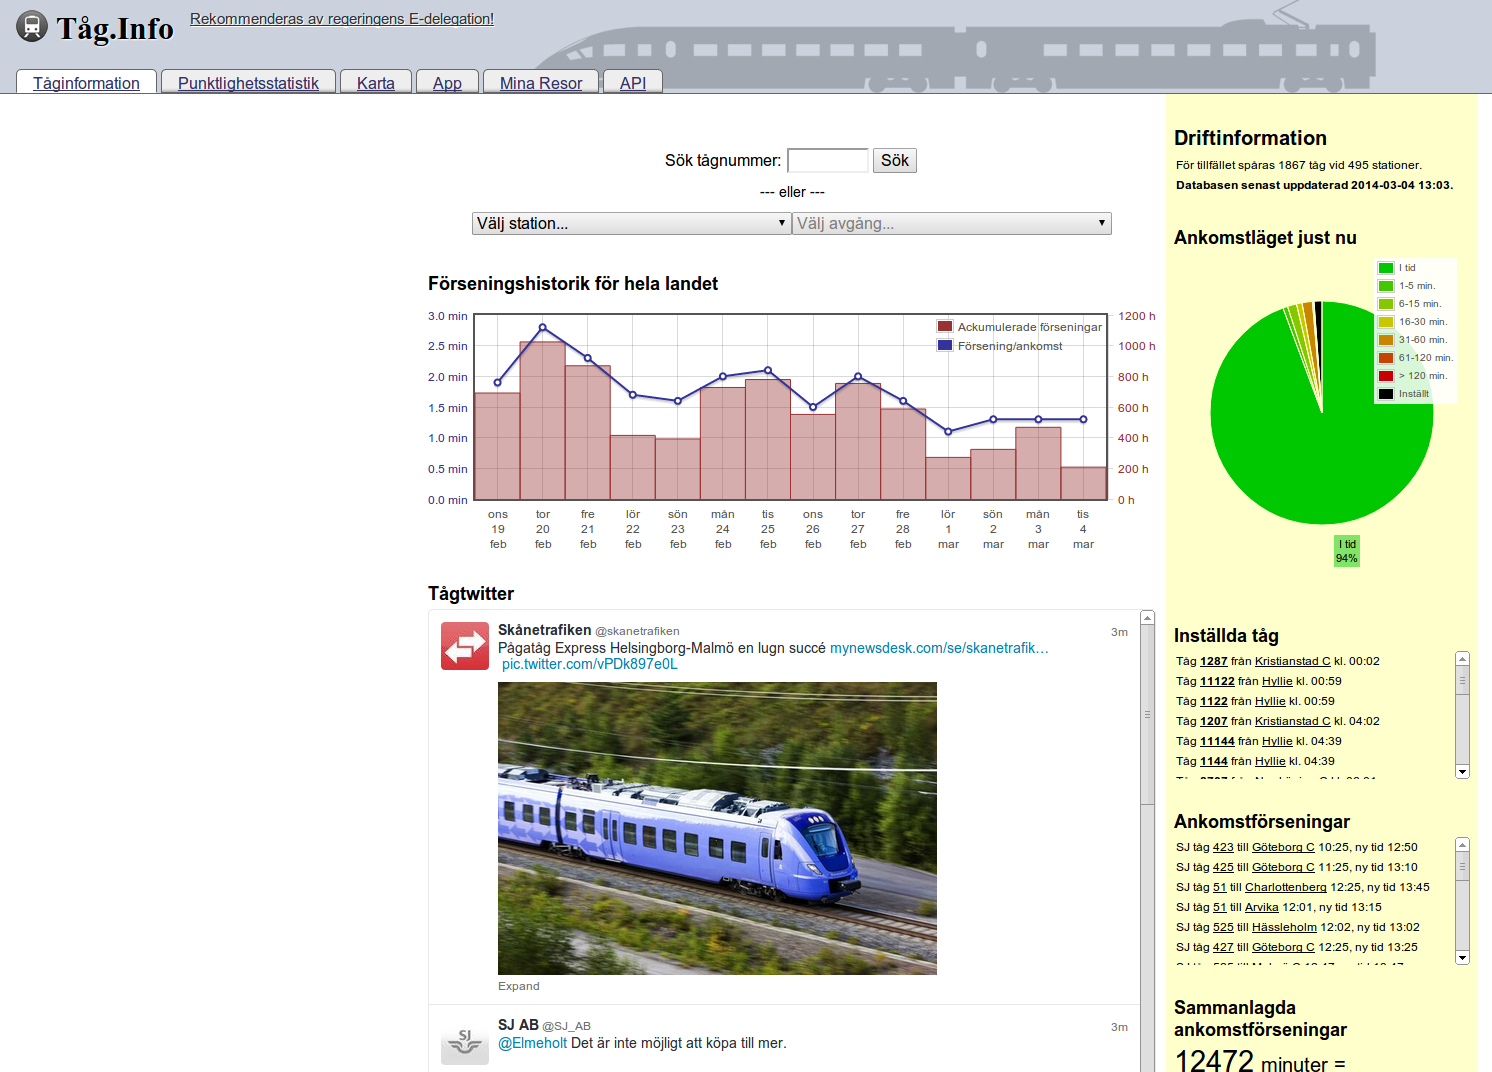
\includegraphics[width=\textwidth,center]{taag-info-historik.png}
	\caption[Tåg.info history]{Tåg.info history
	\cite{taagInfo}}
	\label{fig:taag-info-kart}
\end{figure}
\pagebreak


\subsection{SINTEF Presis}
\label{sub:subsection_sintefPresis}

The PRESIS\cite{sintefPresis} project is a project between SINTEF\cite{sintef},
Transportøkonomisk Institutt\cite{transportOkonomiskInstitutt},
NTNU\cite{ntnu}, Jernbaneverket(section \vref{subsection:jernbaneverket}) and the train operators. It is meant to
systematicly improve the precision level in the railway system by developing
methods, tools, and processes. In this project it has been developed several
prototypes for analyzing train delays. 

If you look at \vref{fig:kjoretidstes-strekning}, it is possible to analyze the
difference in density between two selectable stations on two different,
selectable time periods. 

When looking at \vref{fig:krysningsinteraksjon}, it is possible to see how one
train might affect another at a selected station, plotted based on how much
both trains are delayed from -1 to 20 minutes. 



%\begin{figure}[!htbp]
%	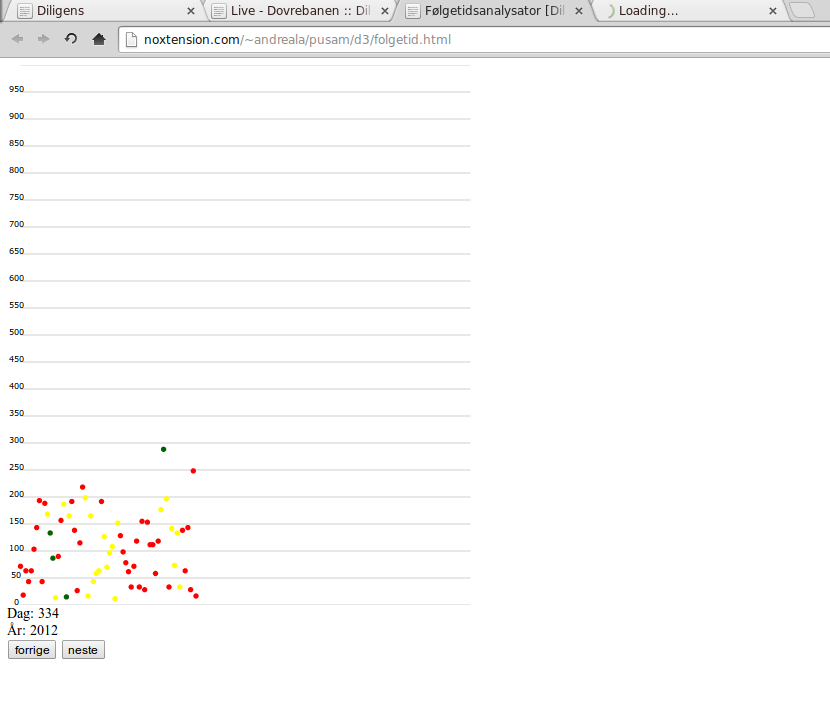
\includegraphics[width=\textwidth,center]{folgetid.png}
%	\caption[folgetid]{folgetid \cite{sintefPresis}}
%	\label{fig:folgetid}
%\end{figure}
%\pagebreak

\begin{figure}[!htbp]
	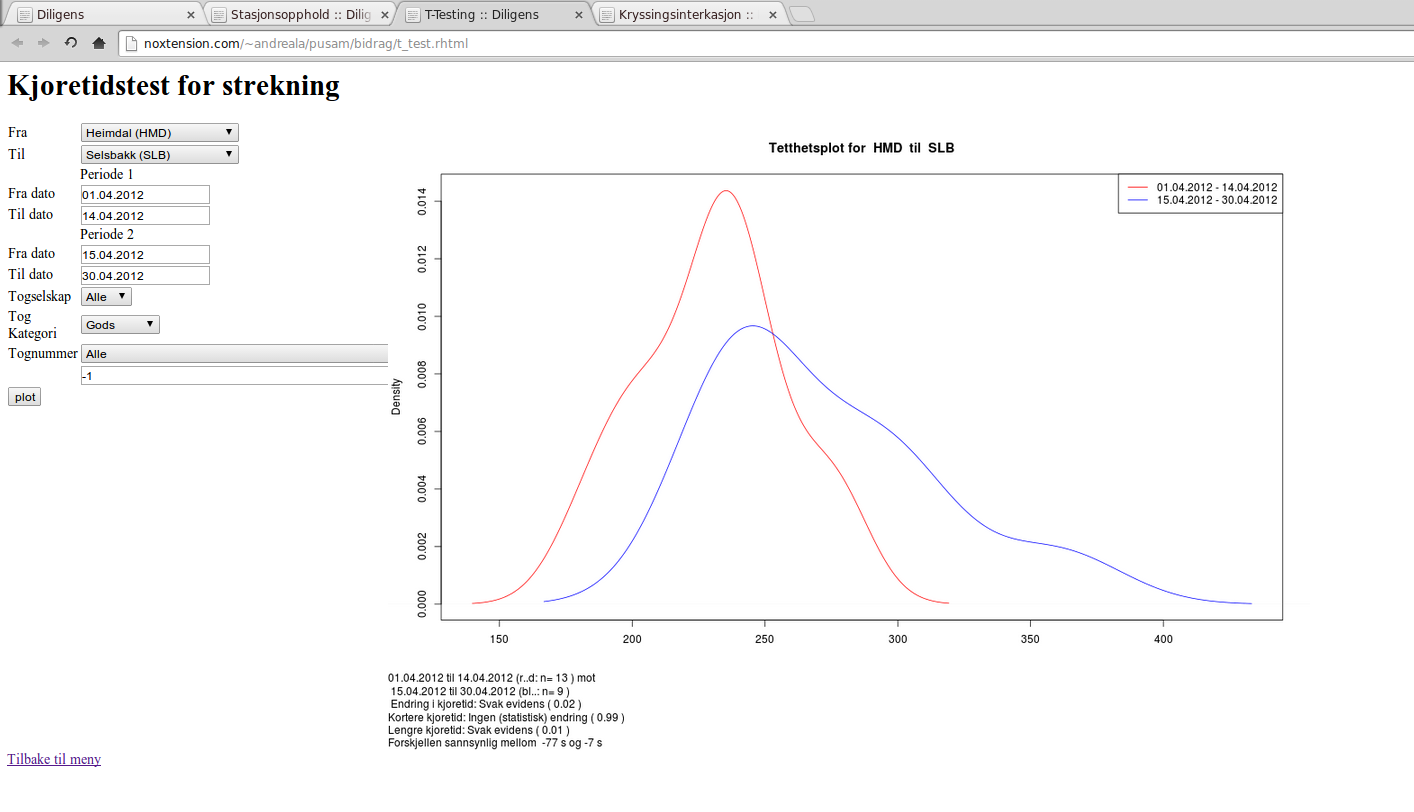
\includegraphics[width=\textwidth,center]{kjoretidstes-strekning.png}
	\caption[Density plot based on driving time]{Density plot based on driving time \cite{sintefPresis}}
	\label{fig:kjoretidstes-strekning}
\end{figure}
\pagebreak

\begin{figure}[!htbp]
	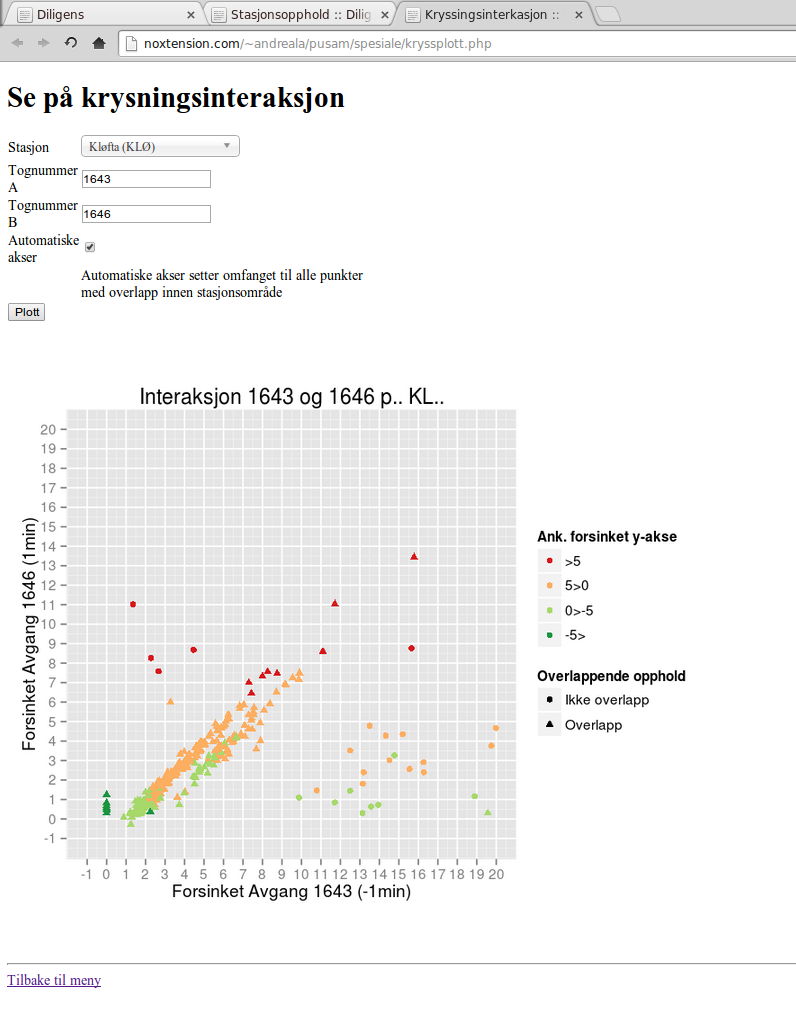
\includegraphics[width=\textwidth,center]{krysningsinteraksjon.png}
	\caption[Train interaction plot]{Train interaction plot \cite{sintefPresis}}
	\label{fig:krysningsinteraksjon}
\end{figure}
\pagebreak

\begin{figure}[!htbp]
	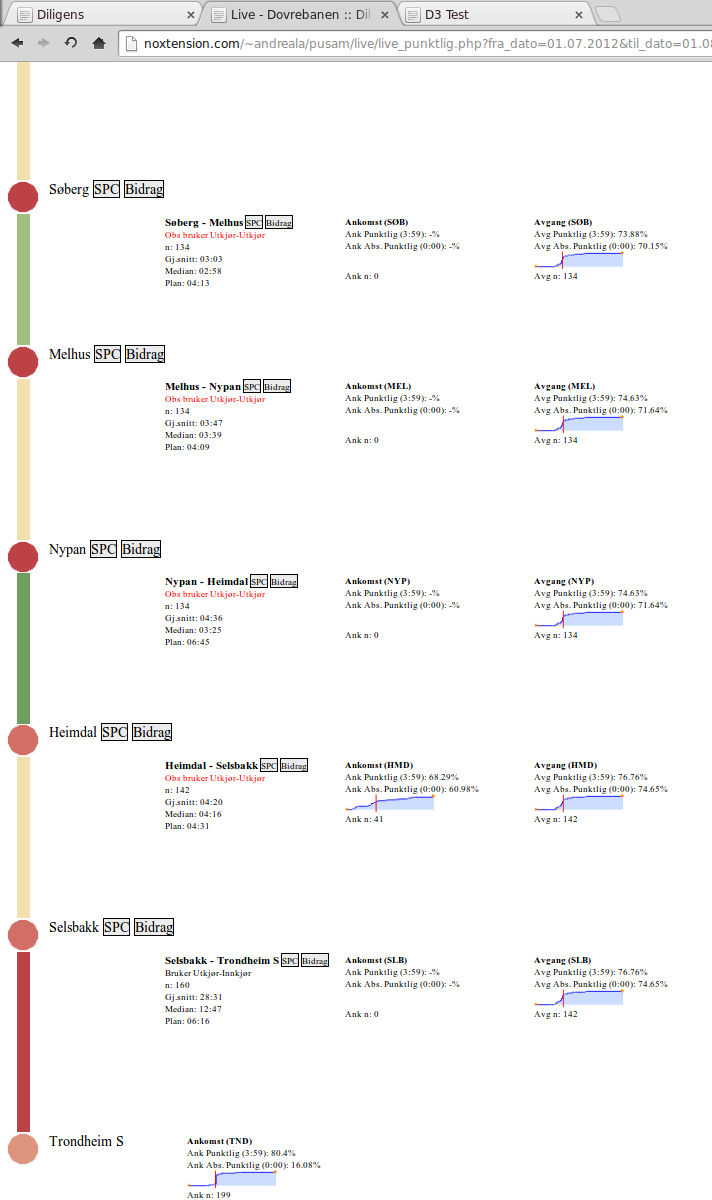
\includegraphics[height=\textheight,center]{live-punklighet.png}
	\caption[Punctuality for routes]{Punctuality for routes \cite{sintefPresis}}
	\label{fig:live-punklighet}
\end{figure}
\pagebreak

\begin{figure}[!htbp]
	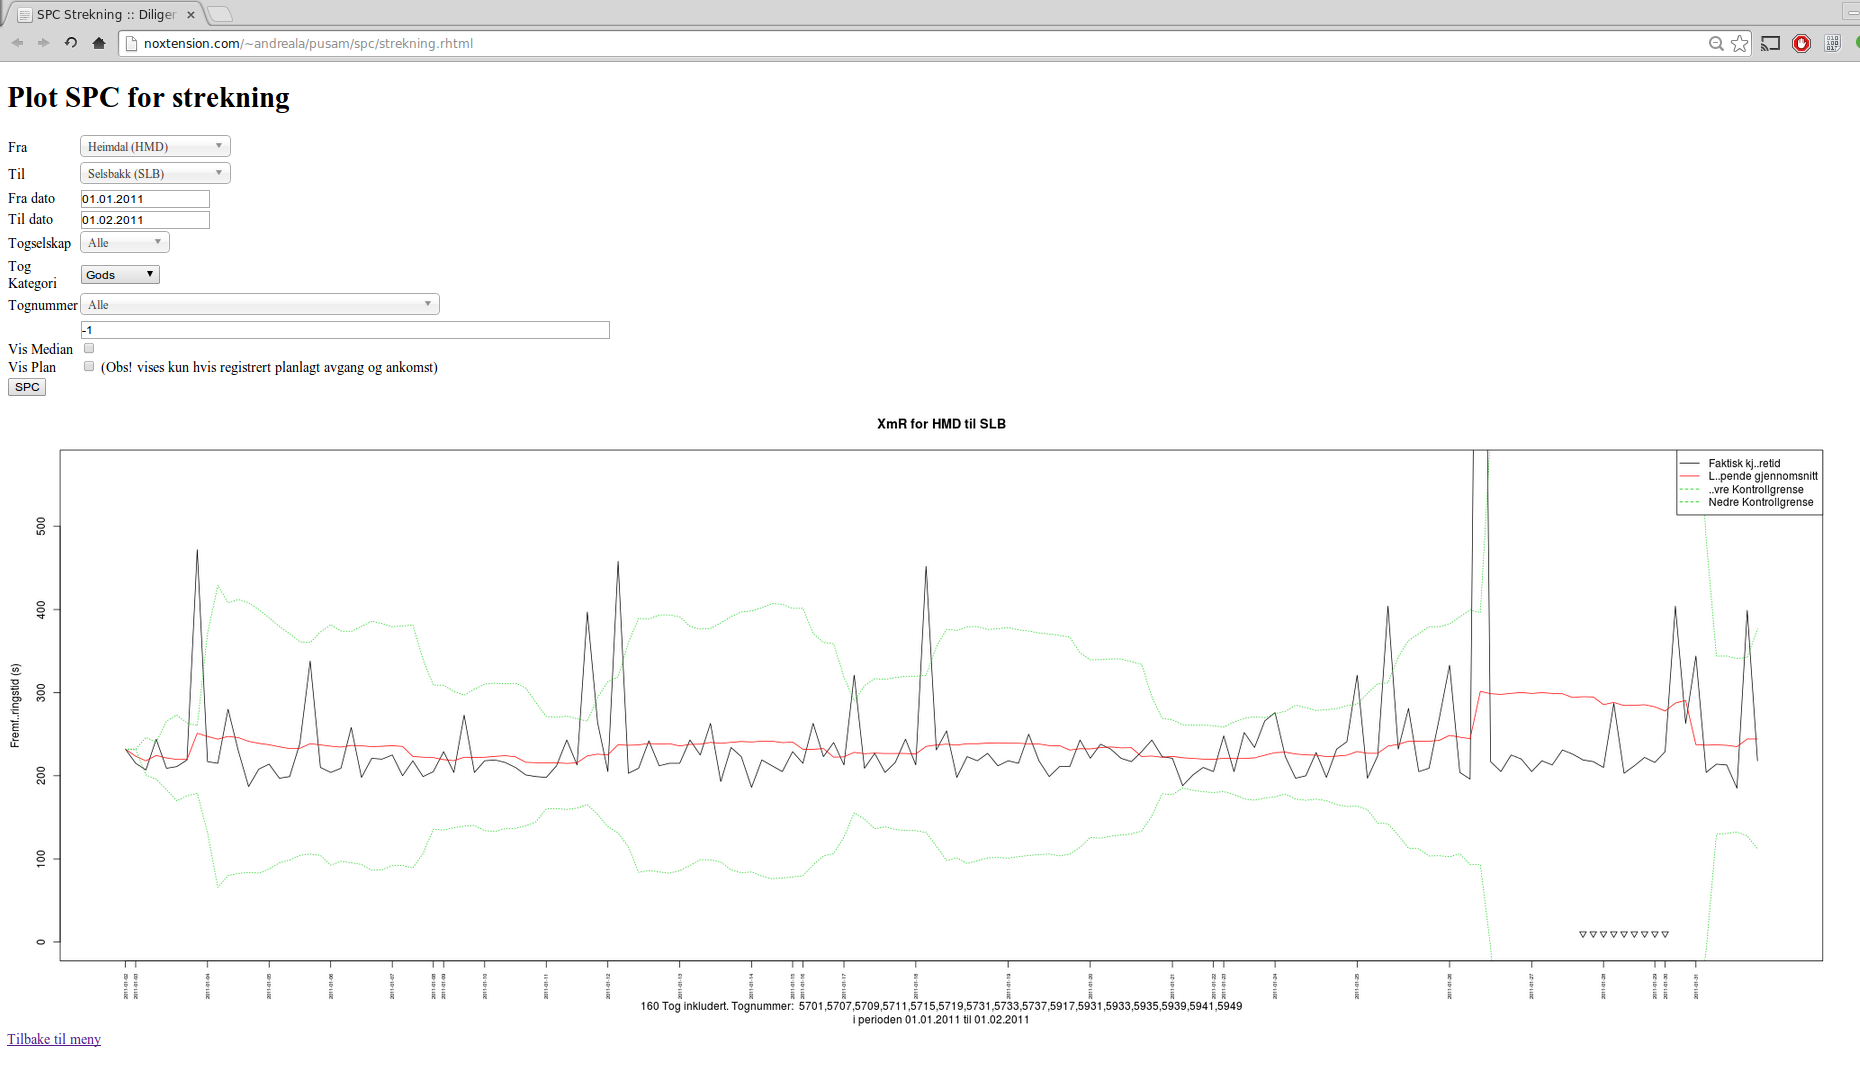
\includegraphics[width=\textwidth,center]{plot-spc-for-strekning.png}
	\caption[Time over distance plot (SPC)]{Time over distance plot (SPC) \cite{sintefPresis}}
	\label{fig:plot-spc-for-strekning}
\end{figure}
\pagebreak

\begin{figure}[!htbp]
	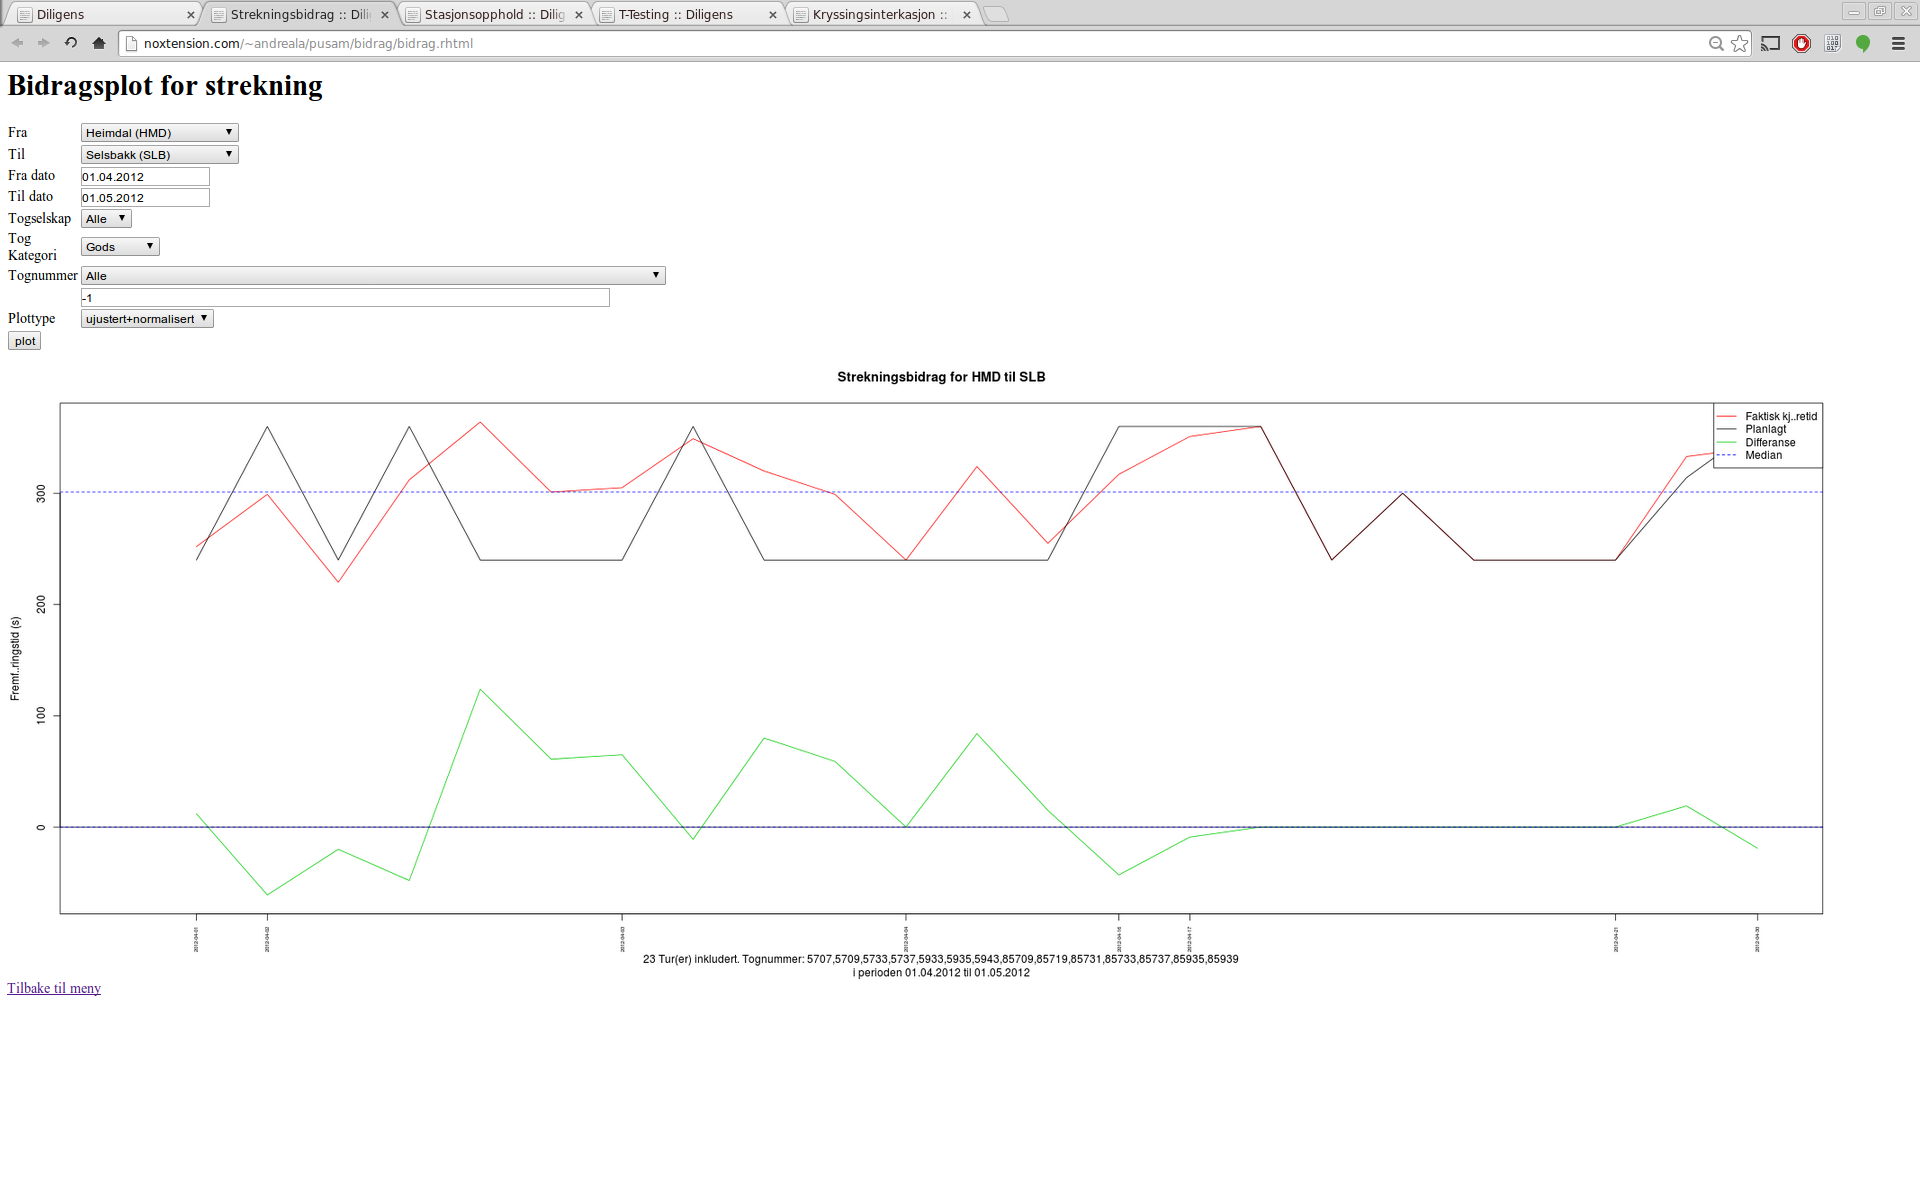
\includegraphics[width=\textwidth,center]{bidragsplot-strekning.png}
	\caption[Time over distance plot (Bidrag)]{Time over distance plot (Bidrag) \cite{sintefPresis}}
	\label{fig:bidragsplot-strekning}
\end{figure}
\pagebreak

\begin{figure}[!htbp]
	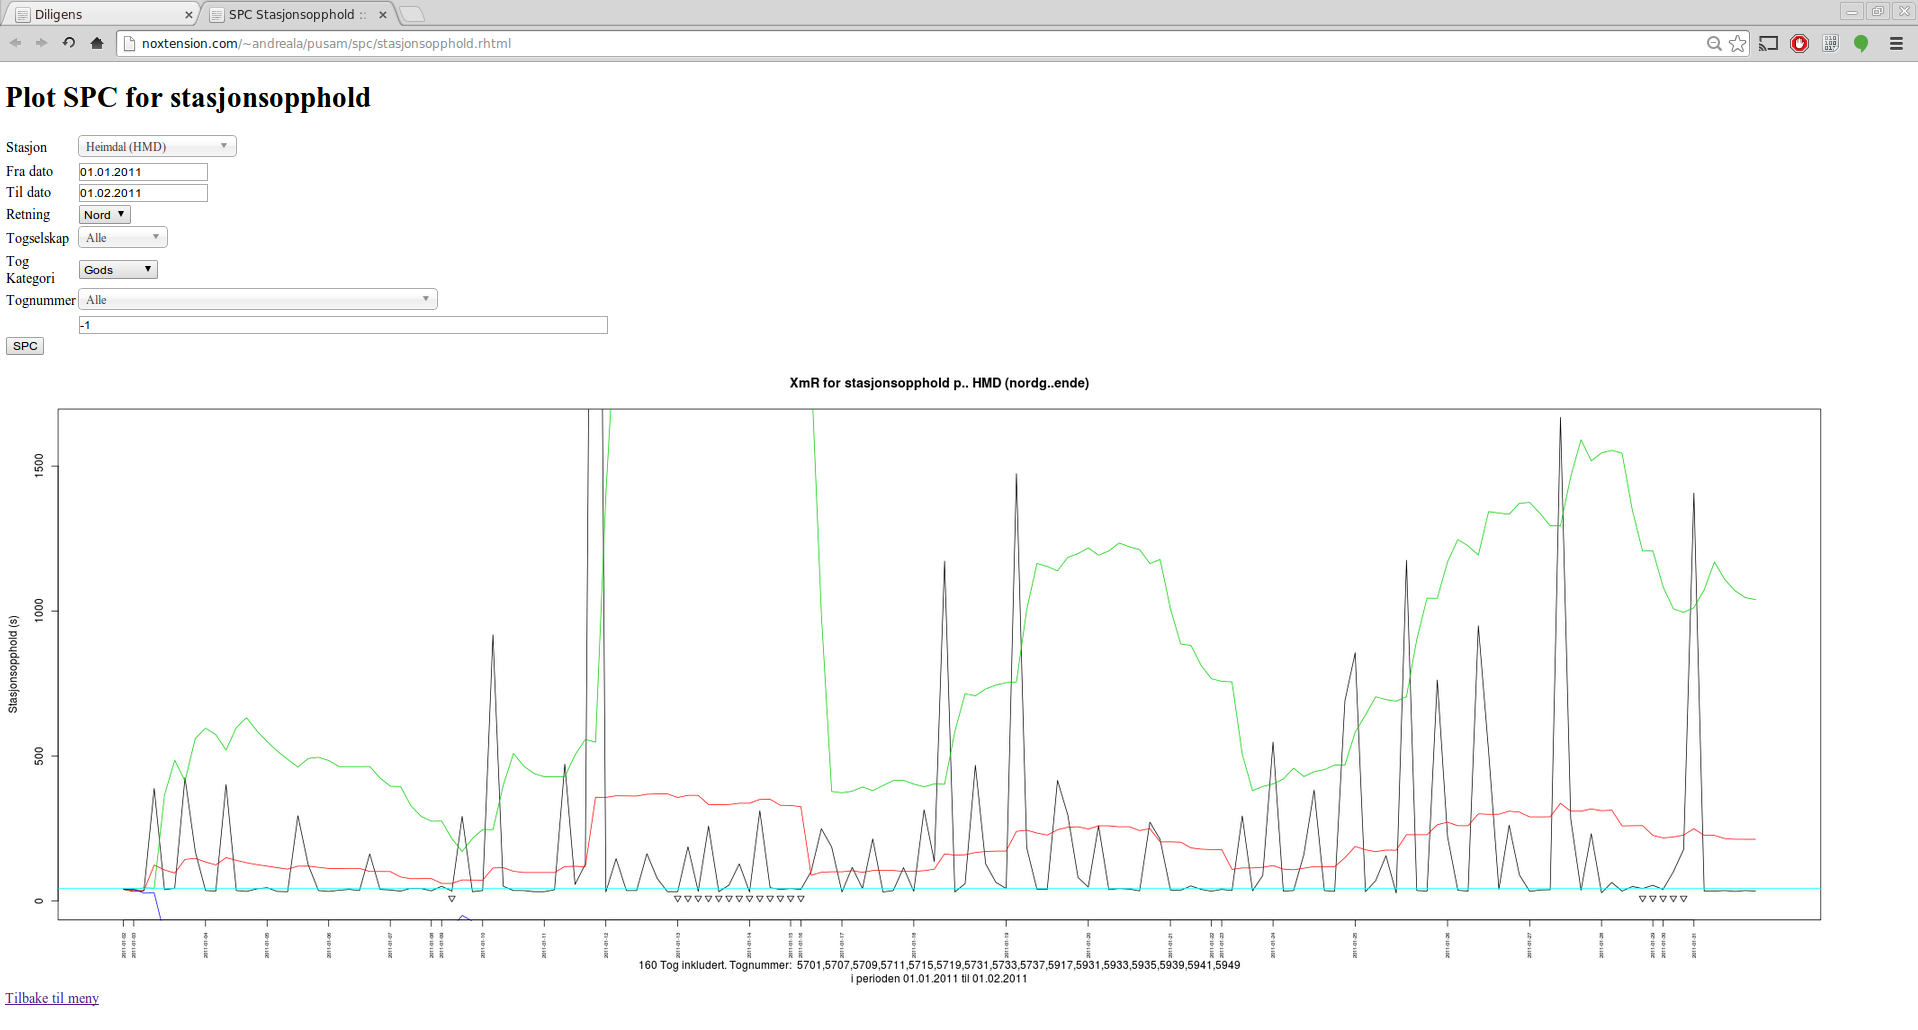
\includegraphics[width=\textwidth,center]{plot-spc-stasjonsopphold.png}
	\caption[Time at station (SPC)]{Time at station (SPC) \cite{sintefPresis}}
	\label{fig:plot-spc-for-stasjonsopphold}
\end{figure}
\pagebreak

\begin{figure}[!htbp]
	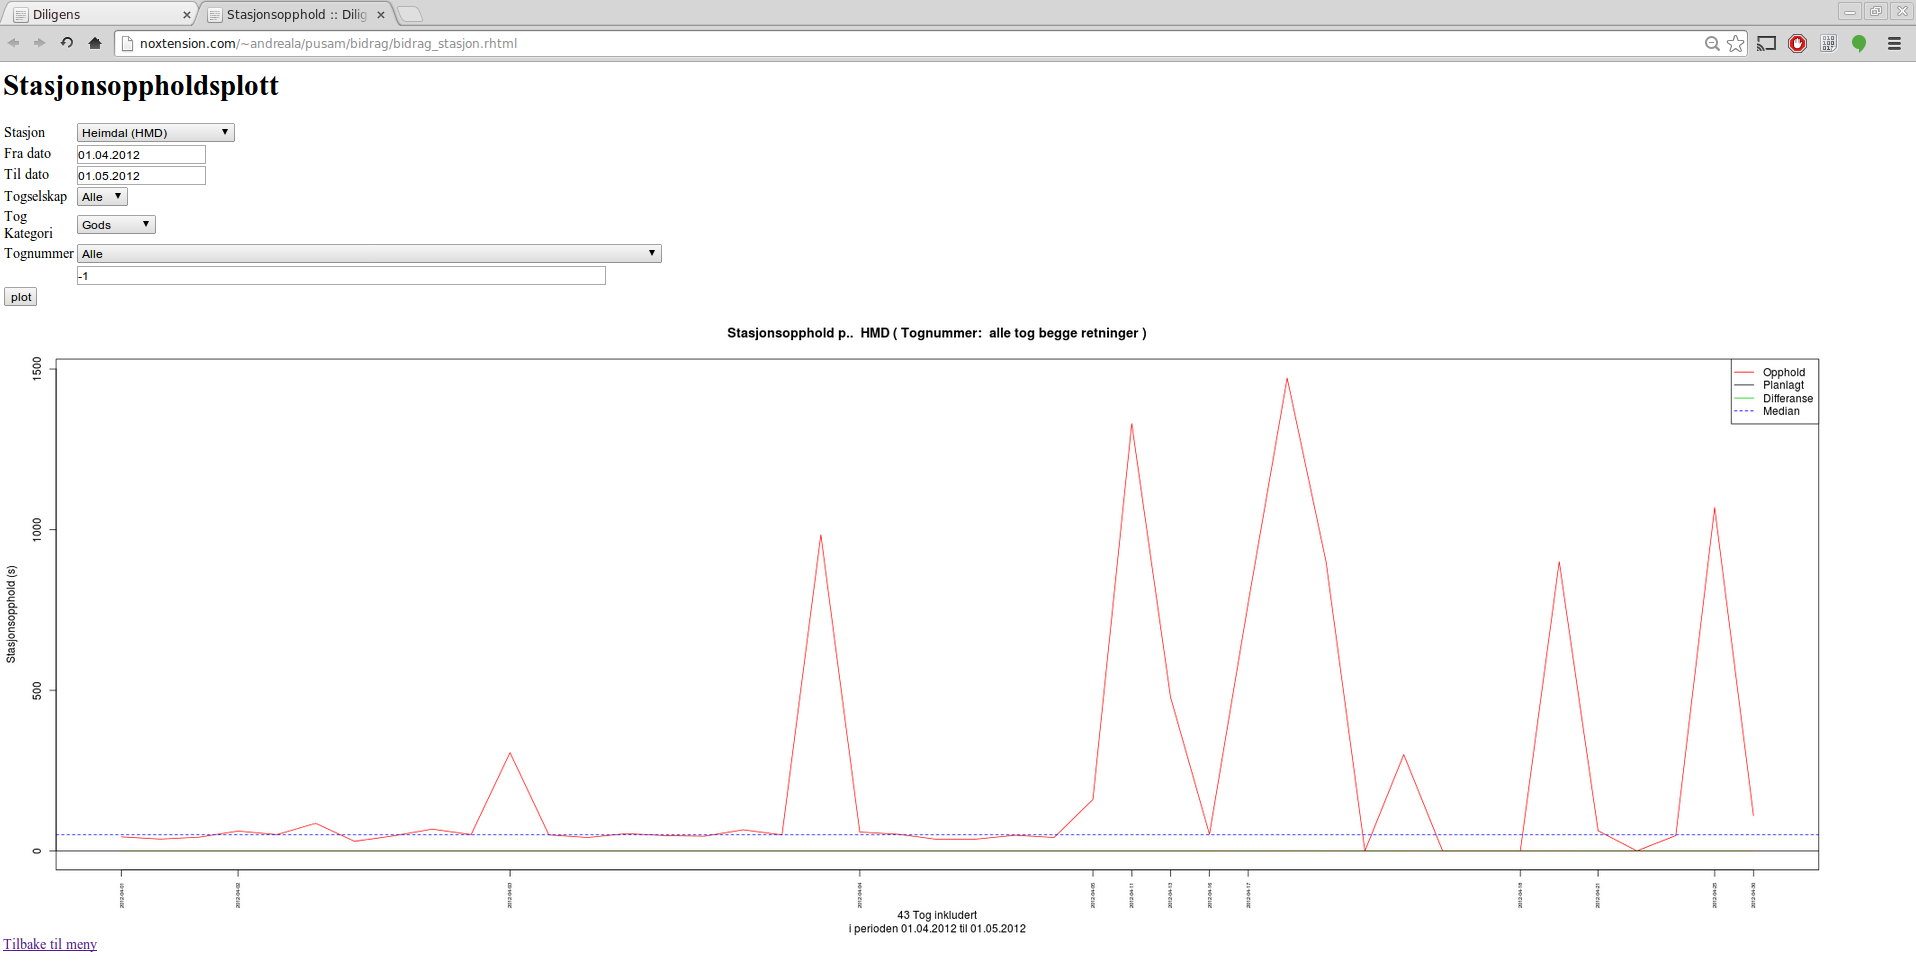
\includegraphics[width=\textwidth,center]{stasjonsoppholdplott.png}
	\caption[Time at station (Bidrag)]{Time at station (Bidrag) \cite{sintefPresis}}
	\label{fig:stasjonsoppholdplott}
\end{figure}
\pagebreak

\begin{figure}[!htbp]
	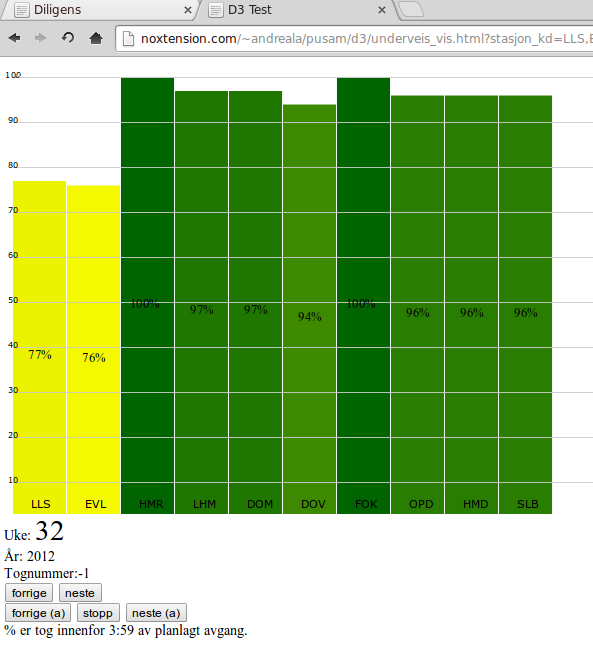
\includegraphics[width=\textwidth,center]{ukespunklighet.png}
	\caption[Weekly punctuality between stations]{Weekly punctuality between stations \cite{sintefPresis}}
	\label{fig:ukespunklighet}
\end{figure}
\pagebreak

\subsection{Cargonet} % (fold)
\label{sub:subsection_cargonet}

% subsection subsection_name (end)
Cargonet is a Norwegian which provides intermodal transport on rails. To 
provide a effective tracking service for the customers, Cargonet provides a 
internal service for the users which tracks all trains belonging to Cargonet.
As can be seen on \vref{fig:cargonet}, it only shows a picture of the current
status of each train, it lacks the possibility to analyze both each stretch 
individually  and analyze trains and stretches in time.

\caption[How to read \ref{fig:cargonet}]{}
\begin{itemize}
	\item Red arrow:\hspace{4ex} Delayed.
	\item White arrow:\hspace{4ex} On time.
	\item Red box:\hspace{4ex} Locomotive driven 2km without carriages.
	\item Black box:\hspace{4ex} Locomotive without carriages.
	\item Yellow box:\hspace{4ex} Locomotive on time without schedule, or known position.
\end{itemize}
}

\begin{figure}[!htbp]
	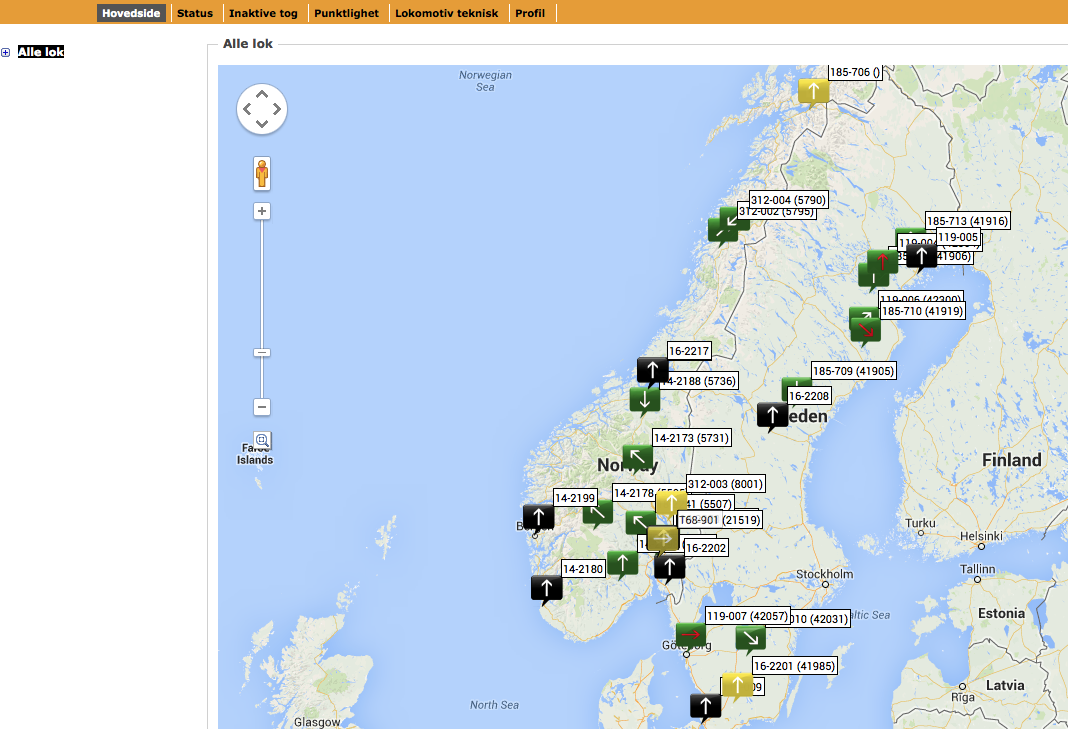
\includegraphics[width=\textwidth,center]{cargonet.png}
	\caption[Cargonet]{Cargonet \cite{cargonet}}
	\label{fig:cargonet}
\end{figure}
\pagebreak
% subsection subsection_cargonet (end)
